\qrchapter{https://forgottenpillar.com/rsc/en-fp-chapter14}{Adventist pioneers and the Trinity doctrine}


\qrchapter{https://forgottenpillar.com/rsc/en-fp-chapter14}{Waanzilishi wa Kiadventista na fundisho la Utatu}


Sister White wrote that early Adventist pioneers \egwinline{are to bear their testimony as to what constitutes the truth for this time}[Lt329-1905.18; 1905][https://egwwritings.org/read?panels=p8455.24] because \egwinline{they have learned to avoid errors and dangers, and are they not then competent to give wise counsel}[7T 287.3; 1902][https://egwwritings.org/read?panels=p117.1637]? In their writings, we see their unanimous views regarding the \emcap{personality of God}, and that they have avoided the Trinitarian error. There is much to write about this topic because the Adventist pioneers left a lot of material dealing directly or indirectly with the doctrine of Trinity. But we will look at some of the testimonies from James White and brother Loughborough because we have read some of their articles on the \emcap{personality of God}. Also, we will compare their testimony with the Spirit of Prophecy as we have done so far.


Dada White aliandika kwamba waanzilishi wa awali wa Waadventista \egwinline{wanapaswa kutoa ushuhuda wao kuhusu yanayojumuisha ukweli kwa wakati huu}[Lt329-1905.18; 1905][https://egwwritings.org/read?panels=p8455.24] kwa sababu \egwinline{wamejifunza kuepuka makosa na hatari, na je, hawana uwezo wa kutoa nasaha zenye hekima}[7T 287.3; 1902][https://egwwritings.org/read?panels=p117.1637]? Katika maandishi yao, tunaona maoni yao ya upamoja kuhusu \emcap{Umbile la Mungu}, na kwamba wameepuka hitilafu ya Utatu. Kuna mengi ya kuandika kuhusu mada hii kwa sababu waanzilishi wa Kiadventista waliacha maandiko mengi yanayohusika moja kwa moja au kwa njia isiyo ya moja kwa moja na fundisho la Utatu. Lakini tutaangalia baadhi ya shuhuda kutoka kwa James White na kaka Loughborough kwa sababu tumesoma baadhi ya makala zao kuhusu \emcap{Umbile la Mungu}. Pia, tutalinganisha ushuhuda wao kwa Roho ya Unabii kama tulivyofanya hadi tulipofikia.


James White, in the Review and Herald, listed \others{some of \textbf{the popular fables} of the age}”, saying: “\others{Here we might mention \textbf{the Trinity, which \underline{does away the personality of God, and of his Son Jesus Christ,} }and of sprinkling or pouring instead of being ‘buried with Christ in baptism,’ ‘planted in the likeness of his death:’ but we pass from these \textbf{fables }to notice one that is held sacred by nearly all professed Christians, both Catholic and Protestant. It is, the change of the Sabbath of the fourth commandment from the seventh to the first day of the week.}[James S. White, Review \& Herald, December 11, 1855, p. 85.15][http://documents.adventistarchives.org/Periodicals/RH/RH18551211-V07-11.pdf]


James White, katika Review and Herald, aliorodhesha \others{baadhi ya \textbf{hekaya maarufu} za enzi hizo}”, akisema: “\others{Hapa tunaweza kutaja \textbf{Utatu, ambao \underline{huondoa Umbile la Mungu, na wa Mwana wake Yesu Kristo,} }na kunyunyiza au kumwagiwa badala ya ‘kuzikwa pamoja na Kristo katika ubatizo,’ ‘kupandwa katika mfano wa mauti yake:’ lakini tunapita kutoka kwa \textbf{hadithi hizi }hadi kuona moja ambayo inachukuliwa kuwa wa kitakatifu na karibu wote wanaodai kuwa Wakristo, Wakatoliki na pia Kiprotestanti. Ni, mabadiliko ya Sabato ya amri ya nne kutoka siku ya saba hadi siku ya kwanza ya juma.}[James S. White, Review \& Herald, December 11, 1855, p. 85.15][http://documents.adventistarchives.org/Periodicals/RH/RH18551211-V07-11.pdf]


What does James White mean when he says that the Trinity \others{does away with the personality of God, and of his Son Jesus Christ}? In Day Star, he wrote:


James White anamaanisha nini anaposema kwamba Utatu \others{huondoa Umbile la Mungu, na wa Mwana wake Yesu Kristo}? Katika Day Star, aliandika:


\others{…a certain class who \textbf{deny the only Lord God and our Lord Jesus Christ}. This class can be no other than those who \textbf{spiritualize away the existence of the Father and the Son}, \textbf{as \underline{two distinct}, \underline{literal}, \underline{tangible persons}}, also a literal Holy city and throne of David… The way spiritualizers this way have disposed of or \textbf{denied the only Lord God and our Lord Jesus Christ is first using \underline{the old unscriptural trinitarian creed}}, viz, that Jesus Christ is the eternal God, though they have not one passage to support it, while we have plain scripture testimony in abundance \textbf{that He is the Son of the eternal God.}}[James White, Day Star, Jan 24, 1846][https://m.egwwritings.org/en/book/741.25\#27]


\others{…kundi fulani ambalo \textbf{linamkana Bwana Mungu pekee na Bwana wetu Yesu Kristo}. Kundi hili haliwezi kuwa lingine zaidi ya wale ambao \textbf{hufanya kuwa ya kiroho kuondoa uwepo wa Baba na Mwana}, \textbf{kama \underline{Nafsi mbili tofauti}, \underline{halisi}, \underline{zinazoonekana}}, pia mji halisi wa Mungu na kiti cha enzi cha Daudi... Njia ambayo wanaofanya mambo kuwa ya kiroho wamefanya kuondoa au \textbf{kumkana Bwana Mungu pekee na Bwana wetu Yesu Kristo ni kwanza kutumia \underline{kanuni ya zamani ya utatu isiyo ya kimaandiko}}, yaani, kwamba Yesu Kristo ni Mungu wa milele, ingawa hawana kifungu hata kimoja cha kuunga mkono, wakati tuna ushuhuda wa maandiko wazi kwa wingi \textbf{kwamba Yeye ni Mwana wa Mungu wa milele.}}[James White, Day Star, Jan 24, 1846][https://m.egwwritings.org/en/book/741.25\#27]


Doing away with the personality of God and His Son is accomplished by denying Them as two distinct, literal, and tangible persons. The doctrine on the personality of God teaches that the Father has a literal, \textit{tangible} person.


Kuondoa Umbile la Mungu na Mwana wake kunafanyika kwa kuwakana Wao kama Nafsi mbili tofauti, halisi, na zinazoonekana. Fundisho juu ya Umbile la Mungu linafundisha kwamba Baba ana nafsi halisi, \textit{inayoonekana}.


In the Adventist Review and Sabbath Herald article from April 4, 1854, James White listed 10 points of \textit{Catholic reasons for keeping Sunday}”, where he said that the Sunday \others{is a day dedicated by the apostles to \textbf{the honor of the most Holy Trinity}}[The Advent Review, and Sabbath Herald, vol. 5 April 4, 1854, p. 86][https://egwwritings.org/read?panels=p1643.2867]. Here we also see the harmony between J. B. Frisbie and James White in their view that the Sabbath is dedicated to the biblical God expressed in the first point of the \emcap{Fundamental Principles}, and Sunday is dedicated to the trinity God. The main problem with the Trinity doctrine is that it \others{does away the personality of God, and of his Son Jesus Christ}. In Life Incidents, he wrote more about why this is so.


Katika makala ya Adventist Review and Sabbath Herald kutoka Aprili 4, 1854, James White aliorodhesha hoja 10 za \textit{sababu za Kikatoliki za kutunza Jumapili}”, ambapo alisema kwamba Jumapili \others{ni siku iliyotengwa na mitume kwa \textbf{heshima ya Utatu Aliye Mtakatifu zaidi}}[The Advent Review, and Sabbath Herald, vol. 5 April 4, 1854, p. 86][https://egwwritings.org/read?panels=p1643.2867]. Hapa tunaona pia maelewano kati ya J. B. Frisbie na James White kwa maoni yao kwamba Sabato imewekwa wakfu kwa Mungu wa kibiblia Aliyeonyeshwa katika hoja ya kwanza ya \emcap{Kanuni za Msingi}, na Jumapili ni wakfu kwa Mungu wa utatu. Tatizo kuu la fundisho la Utatu ni kwamba \others{huondoa Umbile la Mungu, na wa Mwanawe Yesu Kristo}. Katika Life Incidents, aliandika zaidi kuhusu kwa nini hii ni hivyo.


\others{\textbf{Jesus prayed that his disciples might be one as he was \underline{one with his Father}}. \textbf{This prayer did not contemplate one disciple with twelve heads, but twelve disciples, made one in object and effort in the cause of their Master}. \textbf{\underline{Neither are the Father and the Son parts of the ‘three-one God.}}’\footnote{The same quotation is found in James White’s book “\textit{The Law and the Gospel}” with one difference. He states, “\textit{Neither are the Father and the Son parts of \underline{one being}}”; in “\textit{Life Incidents}”, he wrote “parts of the ‘\underline{three-one God}’”. See \href{https://egwwritings.org/?ref=en_LAGO.1.2&para=1492.10}{James S. White, The Law and the Gospel p. 1.2}.} \textbf{\underline{They are two distinct beings}}, \textbf{yet one in the design and accomplishment of redemption}. The redeemed, from the first who shares in the great redemption, to the last, all ascribe the honour, and glory, and praise, of their salvation, to \textbf{both God and the Lamb}.}[James S. White, Life Incidents, p.343.2][https://egwwritings.org/read?panels=p1462.1743]


\others{\textbf{Yesu alisali kwamba wanafunzi wake wawe kitu kimoja kama alivyokuwa \underline{mmoja na Baba yake}}. \textbf{Maombi haya hayakuwaza mfuasi mmoja mwenye vichwa kumi na viwili, bali wanafunzi kumi na wawili, waliofanywa moja kwa lengo na juhudi katika njia ya Bwana wao}. \textbf{\underline{Wala Baba na Mwana si sehemu za ‘Mungu watatu-mmoja.}}’\footnote{Nukuu hiyo hiyo inapatikana katika kitabu cha James White “\textit{The Law and the Gospel}” na tofauti moja. Anasema, “\textit{Wala Baba na Mwana si sehemu za \underline{huluki moja}}”; katika “\textit{Life Incidents}”, aliandika “sehemu za ‘\underline{Mungu watatu-mmoja}’“. Tazama \href{https://egwwritings.org/?ref=en_LAGO.1.2&para=1492.10}{James S. White, The Law and the Gospel p. 1.2}.} \textbf{\underline{Wao ni Nafsi mbili tofauti}}, \textbf{lakini mmoja katika muundo na utimilifu wa ukombozi}. Waliokombolewa, kutoka kwa wa kwanza ambaye anashiriki katika ukombozi mkuu, hadi wa mwisho, wote wanapeana heshima, na utukufu, na sifa, za wokovu wao, \textbf{Mungu na Mwanakondoo pia}.}[James S. White, Life Incidents, p.343.2][https://egwwritings.org/read?panels=p1462.1743]


Sister White wrote similarly regarding Christ’s prayer:


Dada White aliandika vile vile kuhusu sala ya Kristo:


\egw{The burden of that prayer was that His disciples might be \textbf{one as He was one with the Father}; the oneness so close that, \textbf{although \underline{two distinct beings}}, there was \textbf{perfect unity of spirit, purpose, and action}. The mind of the Father was the mind of the Son.}[Lt1-1882.1; 1882][https://egwwritings.org/read?panels=p4120.5]


\egw{Mzigo wa maombi hayo ulikuwa kwamba wanafunzi Wake wawe \textbf{kitu kimoja kama vile Yeye alivyokuwa Mmoja na Baba}; umoja uliokaribi-ana hivi kwamba, \textbf{ingawa walikuwa \underline{Nafsi wawili tofauti}}, kulikuwa na \textbf{umoja kamili ya roho, kusudi, na vitendo}. Nia ya Baba ilikuwa nia ya Mwana.}[Lt1-1882.1; 1882][https://egwwritings.org/read?panels=p4120.5]


\egw{\textbf{The unity that exists between Christ and His disciples \underline{does not destroy the personality of either}}. They are one in purpose, in mind, in character, \textbf{but \underline{not in person}}. \textbf{It is thus that God and Christ are one}.}[MH, 421 422; 1905][https://egwwritings.org/read?panels=p135.2177]


\egw{\textbf{Umoja uliopo kati ya Kristo na wanafunzi wake \underline{hauharibu ubinafsi wa kila mmoja}}. Wao ni wamoja kwa kusudi, akilini, katika tabia, \textbf{lakini \underline{sio kibinafsi}}. \textbf{Ni hivyo kwamba Mungu na Kristo ni mmoja}.}[MH, 421 422; 1905][https://egwwritings.org/read?panels=p135.2177]


The Father and the Son do not comprise one person nor being. The Father and the Son are one, just as Christ and His disciples are one—one in spirit, purpose, mind, and character.


Baba na Mwana hawajumuishi nafsi mmoja wala huluki. Baba na Mwana ni mmoja, kama vile Kristo na wanafunzi Wake ni wamoja—wamoja katika roho, kusudi, akili, na tabia.


Many Adventist trinitarian scholars charge James White and other early pioneers for arianism or semi-arianism, claiming that they made Christ inferior to the Father. This is not true. Let us read the testimony of James White on this matter.


Wataalamu wengi wa utatu wa Waadventista wanamtoza James White na waanzilishi wengine wa mapema uariani au nusu-ariani, wakidai kwamba walimfanya Kristo kuwa duni kwa Baba. Hii si kweli. Hebu tusome ushuhuda wa James White juu ya jambo hili.


\others{Paul affirms of \textbf{the Son of God that he was in the form of God}, and that \textbf{\underline{he was equal with God}}. ‘\textbf{Who being in the form of God thought it not robbery to be \underline{equal with God}}.’ Phil. 2:6. The reason why it is not robbery for the Son \textbf{to be equal with the Father is the fact that he is equal}. If the Son is not equal with the Father, then it is robbery for him to rank himself with the Father.}


\others{Paulo anathibitisha juu ya \textbf{Mwana wa Mungu kwamba alikuwa katika namna ya Mungu}, na kwamba \textbf{\underline{alikuwa sawa na Mungu}}. ‘\textbf{Ambaye kwa kuwa yu yuna namna ya Mungu hakuona kuwa sawa na Mungu kuwa ni kitu cha kushikamana nacho}.’ Fil. 2:6. Sababu kwa nini sio wizi kwa Mwana \textbf{kuwa sawa na Baba ni ukweli kwamba yeye ni sawa}.  Ikiwa Mwana si sawa na Baba, basi ni wizi kwake kuwa na cheo mwenyewe pamoja na Baba.}


\othersnogap{\textbf{\underline{The inexplicable trinity that makes the godhead three in one and one in three, is bad enough}}; \textbf{but that ultra Unitarianism that makes Christ inferior to the Father is worse}. Did God say to an inferior, Let us make man in our image?’}[James S. White, The Advent Review and Sabbath Herald, November 29, 1877, p. 171][https://documents.adventistarchives.org/Periodicals/RH/RH18771129-V50-22.pdf]


\othersnogap{\textbf{\underline{Utatu usioelezeka unaofanya miungu mitatu katika moja na moja katika tatu, ni mbaya kutosha}}; \textbf{lakini imani hiyo ya Unitariani inayomfanya Kristo kuwa duni kwa Baba ni mbaya zaidi}. Je! Mungu alimwambia aliye duni, Na tumfanye mwanadamu kwa mfano wetu?’}[James S. White, The Advent Review and Sabbath Herald, November 29, 1877, p. 171][https://documents.adventistarchives.org/Periodicals/RH/RH18771129-V50-22.pdf]


The problem of the Adventist trinitarian scholars lies in that they themselves cannot completely explain Christ’s divinity other than through the Trinitarian paradigm. Adventist pioneers did believe in Christ’s full divinity but they rejected the Trinity because it destroys the \emcap{personality of God}. \others{The inexplicable trinity that makes the godhead three in one and one in three, \textbf{is bad enough}}. Below is another statement from James White where he compared Seventh-day Adventist with Seventh-day Baptist belief. Seventh-day Adventists did not believe in the Trinity unlike Seventh-day Baptists. James White mentioned that, regarding the divinity of Christ, Seventh-day Adventists hold so nearly with the trinitarian Seventh-day Baptists that they apprehend no trial there.


Tatizo la wataalamu wa utatu wa Kiadventista liko kwa kuwa wao wenyewe hawawezi kueleza kikamilifu uungu wa Kristo zaidi ya kupitia dhana ya Utatu. Waadventista waanzilishi waliamini katika uungu kamili wa Kristo lakini walikataa Utatu kwa sababu unaharibu \emcap{ubinafsi wa Mungu}. \others{Utatu usioelezeka unaofanya miungu mitatu katika moja na moja katika tatu, \textbf{ni mbaya kutosha}}. Chini ni taarifa nyingine kutoka kwa James White ambapo yeye alilinganisha Imani ya Waadventista Wasabato na imani ya Wabaptisti wa Sabato. Waadventista Wasabato hawakuamini Utatu tofauti na Wabaptisti wa Siku ya Saba. James White alisema kuwa, kuhusu uungu wa Kristo, Waadventista Wasabato wanashikilia karibu sana na utatu Wabaptisti wa siku ya saba ambao hawashikilii kesi yoyote kule.


\others{\textbf{The principal difference between the two bodies is the immortality question}. \textbf{The S. D. Adventists hold \underline{the divinity of Christ so nearly with the trinitarian}, that we apprehend no trial here}. And as the practical application of the subject of the Gifts of the Spirit to our people and to our work is better understood by our S. D. Baptist brethren, they manifest less concern for us on this account.}[James S. White, The Advent Review and Sabbath Herald, October 12, 1876, p. 116][https://documents.adventistarchives.org/Periodicals/RH/RH18761012-V48-15.pdf]


\others{\textbf{Tofauti kuu kati ya miili miwili ni swali la kutokufa}. \textbf{Shirika la S.D. Waadventista wanashikilia uungu wa Kristo karibu sana na utatu, kwamba tunaufahamu hakuna kesi hapa}. Na kama matumizi ya vitendo kwenye somo la Karama za Roho kwetu watu na kwa kazi yetu inaeleweka vyema na ndugu zetu wa S. D. Baptist, wanadhihirisha kidogo kujali kwetu kwa sababu hii.}[James S. White, The Advent Review and Sabbath Herald, October 12, 1876, p. 116][https://documents.adventistarchives.org/Periodicals/RH/RH18761012-V48-15.pdf]


This evidence should raise questions to each Adventist trinitarian scholar. How could it be that the Adventist pioneers adhere to the divinity of Christ as trinitarians did, yet rejected the Trinity doctrine? In which way was Christ fully divine, if He was not part of an amalgamated three-in-one God? The answer is simple and completely Biblical. Christ is fully divine, just as His Father, because He was begotten in the express image of the Father’s person; thus, He inherited complete divine nature from His Father.


Ushahidi huu unapaswa kuibua maswali kwa kila mwataalamu wa utatu wa Kiadventista. Inawezaje kuwa kwamba waanzilishi wa Kiadventista walishikamana na uungu wa Kristo kama waamini wa utatu walivyofanya, lakini wakakataa fundisho la Utatu? Ni kwa njia gani Kristo alikuwa Mungu kikamilifu, ikiwa hakuwa sehemu ya Mungu aliyeunganishwa watatu katika mmoja? Jibu ni rahisi na la Kibiblia kabisa. Kristo ni Mungu kwa ukamilifu, kama Baba yake, kwa sababu alizaliwa kwa sura ya wazi ya nafsi ya Baba; hivyo, Alirithi asili kamili ya kimungu kutoka kwa Baba Yake.


\egw{A complete offering has been made; for ‘God so loved the world, that he gave his only-begotten Son,’—\textbf{not a son by creation}, as were the angels, nor a son by adoption, as is the forgiven sinner, but \textbf{a Son \underline{begotten} in the express image of the Father’s person}, and in all the brightness of his majesty and glory, \textbf{one equal with God} in authority, dignity, and \textbf{divine perfection}. \textbf{In him dwelt all the fullness of the Godhead bodily}.}[ST May 30, 1895, par. 3; 1895][https://egwwritings.org/read?panels=p820.12891]


\egw{Sadaka kamili imetolewa; kwa maana ‘Mungu aliupenda ulimwengu, hata akatoa wake Mwana pekee,’—\textbf{si mwana kwa kuumbwa}, kama walivyokuwa malaika, wala mwana kwa kufanywa wana, kama ni mwenye dhambi aliyesamehewa, lakini \textbf{Mwana \underline{aliyezaliwa} kwa sura ya wazi ya nafsi ya Baba}, na katika mng'ao wote wa enzi na utukufu wake, \textbf{aliye sawa na Mungu} katika mamlaka, adhama, na \textbf{ukamilifu wa kimungu}. \textbf{Ndani yake unakaa utimilifu wote wa Uungu, kwa jinsi ya kimwili}.}[ST May 30, 1895, par. 3; 1895][https://egwwritings.org/read?panels=p820.12891]


Christ's complete divinity is not based on an amalgamated \emcap{personality of God}, but rather on His Sonship with the Father. The Bible never refers to Christ with the term “\textit{one God}”—only the Father is referred to with the term “\textit{one God}”\footnote{John 17:3; 1. Corinthians 8:6; 1. Timothy 2:5; Ephesians 4:6} \footnote{We study Christ’s complete divinity in-depth  in the second book of the Forgotten Pillar Project - “\textit{Rediscovering the Pillar}”}. Jesus, the Son of God, is fully divine but is not referred to as \others{\textbf{one God}, \textbf{a personal, spiritual being}} in the first point of the \emcap{Fundamental Principles}.


Uungu kamili wa Kristo hautegemei juu ya \emcap{ubinafsi} uliounganishwa wa Mungu, bali juu ya Uwana wake na Baba. Biblia haimrejelei kamwe Kristo kwa neno “Mungu mmoja”—Baba pekee anarejelewa kwa neno “Mungu mmoja”\footnote{Yohana 17:3; 1. Wakorintho 8:6; 1. Timotheo 2:5; Waefeso 4:6} \footnote{Tunasoma uungu kamili wa Kristo kwa kina katika kitabu cha pili cha Mradi wa Nguzo Iliyosahaulika - “Kugundua upya Nguzo”}. Yesu, Mwana wa Mungu, ni Mungu kamili lakini haielezwi kuwa \others{\textbf{Mungu mmoja}, \textbf{huluki wa kibinafsi, wa kiroho}} katika hoja ya kwanza ya \emcap{Kanuni za Msingi}.


\egw{The Lord Jesus Christ, the only begotten Son of the Father, \textbf{is truly God in infinity, \underline{but not in personality}}.}[Ms116-1905.19; 1905][https://egwwritings.org/read?panels=p10633.25]


\egw{Bwana Yesu Kristo, Mwana pekee wa Baba, \textbf{kweli ni Mungu katika ukomo, \underline{lakini sivyo katika ubinafsi}}.}[Ms116-1905.19; 1905][https://egwwritings.org/read?panels=p10633.25]


Brother J. N. Loughborough was asked to answer the question, \others{What serious objection is there to the doctrine of the Trinity?}[The question was asked by Brother W. W. Giles and it was sent to James S. White, who forwarded the question to Brother John N. Loughborough.]. As we read his answer, let us try to understand some of the reasons why the early pioneers did not adhere to this doctrine.


Ndugu J. N. Loughborough aliombwa kujibu swali, \others{Ni upinzani gani zito uko kwenye fundisho la Utatu?}[Swali liliulizwa na Ndugu W. W. Giles na lilipelekwa kwa James S. White, ambaye alipeleka swali hilo kwa Ndugu John N. Loughborough.]. Tunaposoma jibu lake, acheni tujaribu kuelewa baadhi ya sababu kwa nini waanzilishi wa awali hawakushikamana na fundisho hili.


\others{There are many objections which we might urge, but on account of our limited space we shall reduce them to the three following: \textbf{1. It is contrary to common sense. 2. It is contrary to scripture. 3. Its origin is Pagan and fabulous.}}


\others{Kuna pingamizi nyingi ambazo tunaweza kuhimiza, lakini kwa sababu ya nafasi yetu ndogo sisi tutapunguza hadi tatu zifuatazo: \textbf{1. Ni kinyume na akili timamu. 2. Ni kinyume na maandiko. 3. Asili yake ni ya Kipagani na ya ajabu.}}


\othersnogap{These positions we will remark upon briefly in their order. And 1. \textbf{It is not very consonant with common sense to talk of three being one, and one being three}. \textbf{Or as some express it, calling God ‘the Triune God,’ or ‘the three-one-God.’} \textbf{If Father, Son, and Holy Ghost are each God, it would be three Gods; for three times one is not one, but three}. \textbf{\underline{There is a sense in which they are one, but not one person, as claimed by Trinitarians}}}.


\othersnogap{Nafasi hizi tutazieleza kwa ufupi kwa mpangilio wao. Na 1. \textbf{Haina uthabiti na akili timamu kuongelea watatu kuwa Mmoja, na mmoja kuwa watatu}. \textbf{Au kama wengine kulieleza, akimwita Mungu ‘Mungu wa Utatu,’ au ‘Mungu watatu-mmoja.’} \textbf{Ikiwa Baba, Mwana, na Roho Mtakatifu ni kila Mungu, ingekuwa ni Miungu watatu; maana mara tatu mtu si mmoja, lakini tatu}. \textbf{\underline{Kuna hali ambayo wao ni mmoja, lakini sio mtu mmoja, kama inavyodaiwa na Waamini Utatu}}}.


\othersnogap{2. \textbf{It is contrary to Scripture}. \textbf{Almost any portion of the New Testament we may open which has occasion to speak of the Father and Son, represents them as two distinct persons}. \textbf{\underline{The seventeenth chapter of John is alone sufficient to refute the doctrine of the Trinity}}. \textbf{Over forty times in that one chapter Christ speaks of his Father as a person distinct from himself}. His Father was in heaven and he upon earth. The Father had sent him. Given to him those that believed. He was then to go to the Father.\textbf{ And in this very testimony he shows us in what consists the oneness of the Father and Son}.\textbf{\underline{ It is the same as the oneness of the members of Christ’s church}}. ‘\textbf{That \underline{they} all may be one; \underline{as} thou, Father, art in me, and I in thee, \underline{that they also} may be one in us}; that the world may believe that thou hast sent me. And the \textbf{glory which thou gavest me I have given them}; that \textbf{they may be one}, \textbf{even as we are one.}’ \textbf{Of one heart and one mind}. \textbf{Of one purpose} in all the plan devised for man’s salvation. \textbf{\underline{Read the seventeenth chapter of John, and see if it does not completely upset the doctrine of the Trinity}}.}


\othersnogap{2. \textbf{Ni kinyume na Maandiko}. \textbf{Karibu sehemu yoyote ya Agano Jipya tunaweza kufungua ambayo ina nafasi ya kusema juu ya Baba na Mwana, inawawakilisha kama nafsi mbili tofauti}. \textbf{\underline{Sura ya kumi na saba ya Yohana pekee inatosha kukanusha fundisho la Utatu}}. \textbf{Zaidi ya mara arobaini katika sura hiyo moja Kristo anazungumza juu ya Baba yake kama nafsi tofauti na yeye mwenyewe}. Baba yake alikuwa mbinguni na yeye alikuwa duniani. Baba alikuwa amemtuma. Amepewa wale walioamini. Alikuwa basi aende kwa Baba.\textbf{ Na katika ushuhuda huu anaotuonyesha katika kile kinachojumuisha umoja wa Baba na Mwana}.\textbf{\underline{ Ni sawa na umoja wa washiriki wa kanisa la Kristo}}. ‘\textbf{Ili \underline{wote} wawe moja; \underline{kama} wewe, Baba, ulivyo ndani yangu, nami ndani yako, \underline{hao nao} wawe moja ndani yetu}; kwamba ulimwengu upate kusadiki kwamba ndiwe uliyenituma. Na \textbf{utukufu ulionipa nao nawapea}; ili \textbf{wawe kitu kimoja}, \textbf{kama sisi tulivyo umoja.}’ \textbf{Wa moyo mmoja na nia moja}. \textbf{Ya kusudi moja} katika mpango wote uliopangwa kwa ajili ya wokovu wa mwanadamu. \textbf{\underline{Soma sura ya kumi na saba ya Yohana, na uone ikiwa haivunji kabisa fundisho la Utatu}}.}


\othersnogap{\textbf{To believe that doctrine, when reading the scripture we must believe that God sent himself into the world, died to reconcile the world to himself, raised himself from the dead, ascended to himself in heaven, pleads before himself in heaven to reconcile the world to himself, and is the only mediator between man and himself}. It will not do to substitute the human nature of Christ (according to Trinitarians) as the Mediator; for Clarke says, ‘Human blood can no more appease God than swine’s blood.’ Comment on 2 Samuel 21:10. \textbf{We must believe also that in the garden God prayed to himself, if it were possible, to let the cup pass from himself, and a thousand other \underline{such absurdities}}.}


\othersnogap{\textbf{Ili kuamini fundisho hilo, tunaposoma maandiko ni lazima tuamini kwamba Mungu alijituma mwenyewe katika ulimwengu, alikufa ili kuupatanisha ulimwengu na nafsi yake, alijiinua kutoka kwa aliyekufa, akapaa kwake mbinguni, anasihi mbele zake mbinguni ili kupatanisha ulimwengu kwake mwenyewe, na ndiye mpatanishi pekee kati ya mtu na yeye mwenyewe}. Haitafanya kuchukua nafasi ya asili ya kibinadamu ya Kristo (kulingana na waamini Utatu) kama Mpatanishi; kwani Clarke anasema, ‘Damu ya mwanadamu haiwezi kumpendeza Mungu kuliko damu ya nguruwe.’ Fafanua 2 Samweli 21:10. \textbf{Tunapaswa kuamini pia kwamba katika bustani Mungu alijiomba mwenyewe, ikiwa ni ikiwezekana, kukiacha kikombe kipite kutoka kwake mwenyewe, na \underline{upuuzi kama hizo} elfu na elfu}.}


\othersnogap{\textbf{Read carefully the following texts, comparing them with the idea that Christ is the Omnipotent, Omnipresent, Supreme, and only self-existent God: John 14:28; 17:3; 3:16; 5:19, 26; 11:15; 20:19; 8:50; 6:38; Mark 13:32; Luke 6:12; 22:69; 24:29; Matthew 3:17; 27:46; Galatians 3:20; 1 John 2:1; Revelation 5:7; Acts 17:31. Also see Matthew 11:25, 27; Luke 1:32; 22:42; John 3:35, 36; 5:19, 21, 22, 23, 25, 26; 6:40; 8:35, 36; 14:13; 1 Corinthians 15:28, etc}.}


\othersnogap{\textbf{Soma kwa makini maandiko yafuatayo, ukiyalinganisha na wazo kwamba Kristo ndiye Mungu Mwenye Nguvu Zote, Aliyepo Pote, Aliye Juu Zaidi, na pekee anayeishi mwenyewe: Yohana 14:28; 17:3; 3:16; 5:19, 26; 11:15; 20:19; 8:50; 6:38; Marko 13:32; Luka 6:12; 22:69; 24:29; Mathayo 3:17; 27:46; Wagalatia 3:20; 1 Yohana 2:1; Ufunuo 5:7; Matendo 17:31. Pia tazama Mathayo 11:25, 27; Luka 1:32; 22:42; Yohana 3:35, 36; 5:19, 21, 22, 23, 25, 26; 6:40; 8:35, 36; 14:13; 1 Wakorintho 15:28, nk}.}


\othersnogap{\textbf{The word Trinity nowhere occurs in the Scriptures}. \textbf{The principal text supposed to teach it is 1 John 1:7\footnote{J. N. Loughborough made a typo in the original document, he wanted to point out to 1 John 5:7}, which is an interpolation}. Clarke says, ‘\textbf{Out of one hundred and thirteen manuscripts, the text is wanting in one hundred and twelve. It occurs in no MS. before the tenth century. And the first place the text occurs in Greek, is in the Greek translation of the acts of the Council of Lateran, held A. D. 1215}.’ - Comment. on John 1, and remarks at close of chap.}


\othersnogap{\textbf{Neno Utatu halipatikani popote katika Maandiko}. \textbf{Nakala kuu inayopaswa kufundisha ni 1 Yohana 5:7\footnote{J. N. Loughborough alifanya makosa ya uchapishaji katika hati asili, alitaka kuonyesha 1 Yohana 5:7}, ambayo ni tafsiri}. Clarke anasema, ‘\textbf{Kati ya mia moja na kumi na tatu, maandishi hayapo katika mia moja na kumi na mbili. Inatokea katika muswada wowote kabla ya karne ya kumi. Na mahali pa kwanza maandishi yanapatikana katika Kigiriki, ni katika Tafsiri ya Kigiriki ya matendo ya Mtaguso wa Laterani, uliofanyika A. D. 1215}.’ - Maoni. juu Yohana 1, na maelezo mwishoni mwa sura.}


\othersnogap{3. \textbf{Its origin is pagan and fabulous}. Instead of pointing us to scripture for proof of the trinity, we are pointed to the trident of the Persians, with the assertion that by this they designed to teach the idea of a trinity, and if they had the doctrine of the trinity, they must have received it by tradition from the people of God. \textbf{But this is all assumed, for it is certain that the Jewish church held to no such doctrine. Says Mr. Summerbell, ‘A friend of mine who was present in a New York synagogue, asked the Rabbi for an explanation of the \underline{word ’elohim’}. A Trinitarian clergyman who stood by, replied, ‘Why, that has \underline{reference to the three persons in the Trinity},’ when a Jew stepped forward and said he must not mention that word again, or they would have to compel him to leave the house; \underline{for it was not permitted to mention the name of any strange god in the synagogue}.’}\footnote{Discussion between Summerbell and Flood on Trinity, p.38.} Milman says the idea of the Trident is fabulous. (Hist. Christianity, p.34.)}


\othersnogap{3. \textbf{Asili yake ni ya Kipagani na ya ajabu}. Badala ya kutuelekeza kwenye maandiko kwa uthibitisho wa utatu, tunaelekezwa kwenye utatu wa Waajemi, kwa madai kwamba kwa hili wao iliyoundwa kufundisha wazo la utatu, na ikiwa walikuwa na fundisho la utatu, lazima wameipokea kwa mapokeo kutoka kwa watu wa Mungu. \textbf{Lakini hii yote inachukuliwa, kwa kuwa ni hakika kwamba kanisa la Kiyahudi halikushikilia fundisho kama hilo. Anasema Bw. Summerbell, ‘Rafiki yangu ambaye alikuwepo katika sinagogi la New York, alimwomba Rabi ufafanuzi wa \underline{neno ‘elohim’}. Kasisi mmoja wa Utatu aliyesimama karibu, alijibu, ‘Kwa nini, hilo linarejelea \underline{nafsi tatu katika Utatu},’ Myahudi aliposonga mbele na akasema hana budi kutotaja neno hilo tena, la sivyo watalazimishwa kumfanya aondoke chumbani; \underline{kwa maana haikuruhusiwa kutaja jina la mungu yeyote wa ajabu ndani ya sinagogi}.}’\footnote{Discussion between Summerbell and Flood on Trinity, p.38.} Milman anasema wazo la Utatu ni la ajabu. (Hist. Christianity, p.34.)}


\othersnogap{\textbf{This doctrine of the trinity was brought into the church about the same time with image worship, and keeping the day of the sun, and is but Persian doctrine remodeled}. \textbf{It occupied about three hundred years from its introduction to bring the doctrine to what it is now. It was commenced about 325 A. D., and was not completed till 681.} See Milman’s Gibbon’s Rome, vol. iv, p.422. It was adopted in Spain in 589, in England in 596, in Africa in 534. - Gib. vol. iv, pp.114,345; Milner, vol. i, p.519.}[John N. Loughborough, The Adventist Review, and Sabbath Herald, November 5, 1861, p. 184][https://egwwritings.org/read?panels=p1685.6615]


\othersnogap{\textbf{Fundisho hili la utatu lililetwa kanisani karibu wakati huo huo wa kuabudu sanamu, na kushika siku ya jua, na ni mafundisho ya Kiajemi tu imerekebishwa}. \textbf{Ilichukua takriban miaka mia tatu tangu kuanzishwa kwake kuleta fundisho la jinsi lilivyo sasa. Ilianza mnamo 325 A.D., na haikukamilika hadi 681.} Tazama Milman's Gibbon's Rome, juz. iv, uk.422. Ilipitishwa nchini Uhispania mnamo 589, mnamo Uingereza mwaka 596, katika Afrika katika 534. - Gib. juzuu ya iv, uk.114,345; Milner, juzuu. i, uk.519.}[John N. Loughborough, The Adventist Review, and Sabbath Herald, November 5, 1861, p. 184][https://egwwritings.org/read?panels=p1685.6615]


Brother Loughborough was the son of a Methodist minister and he was raised with the belief in the doctrine of Trinity. Besides the reasons he mentioned, he does not adhere to this doctrine because it is not in harmony with the truth on the \emcap{personality of God}. The seventeenth chapter of John is in harmony with the truth on the \emcap{personality of God} taught and practiced by the Seventh-day Adventists; the Trinity doctrine is not.


Ndugu Loughborough alikuwa mwana wa mhudumu wa Methodisti na alilelewa na imani hiyo katika fundisho la Utatu. Kando na sababu alizotaja, yeye hazingatii hili fundisho kwa sababu halipatani na kweli juu ya Umbile la Mungu. Sura ya kumi na saba ya Yohana haikubaliani na fundisho hili kwa sababu haikubaliani na Ukweli kuhusu Umbile la Mungu unaofundishwa na kufanywa na Waadventista Wasabato; fundisho la Utatu si.


\begin{figure}[hp]
    \centering
    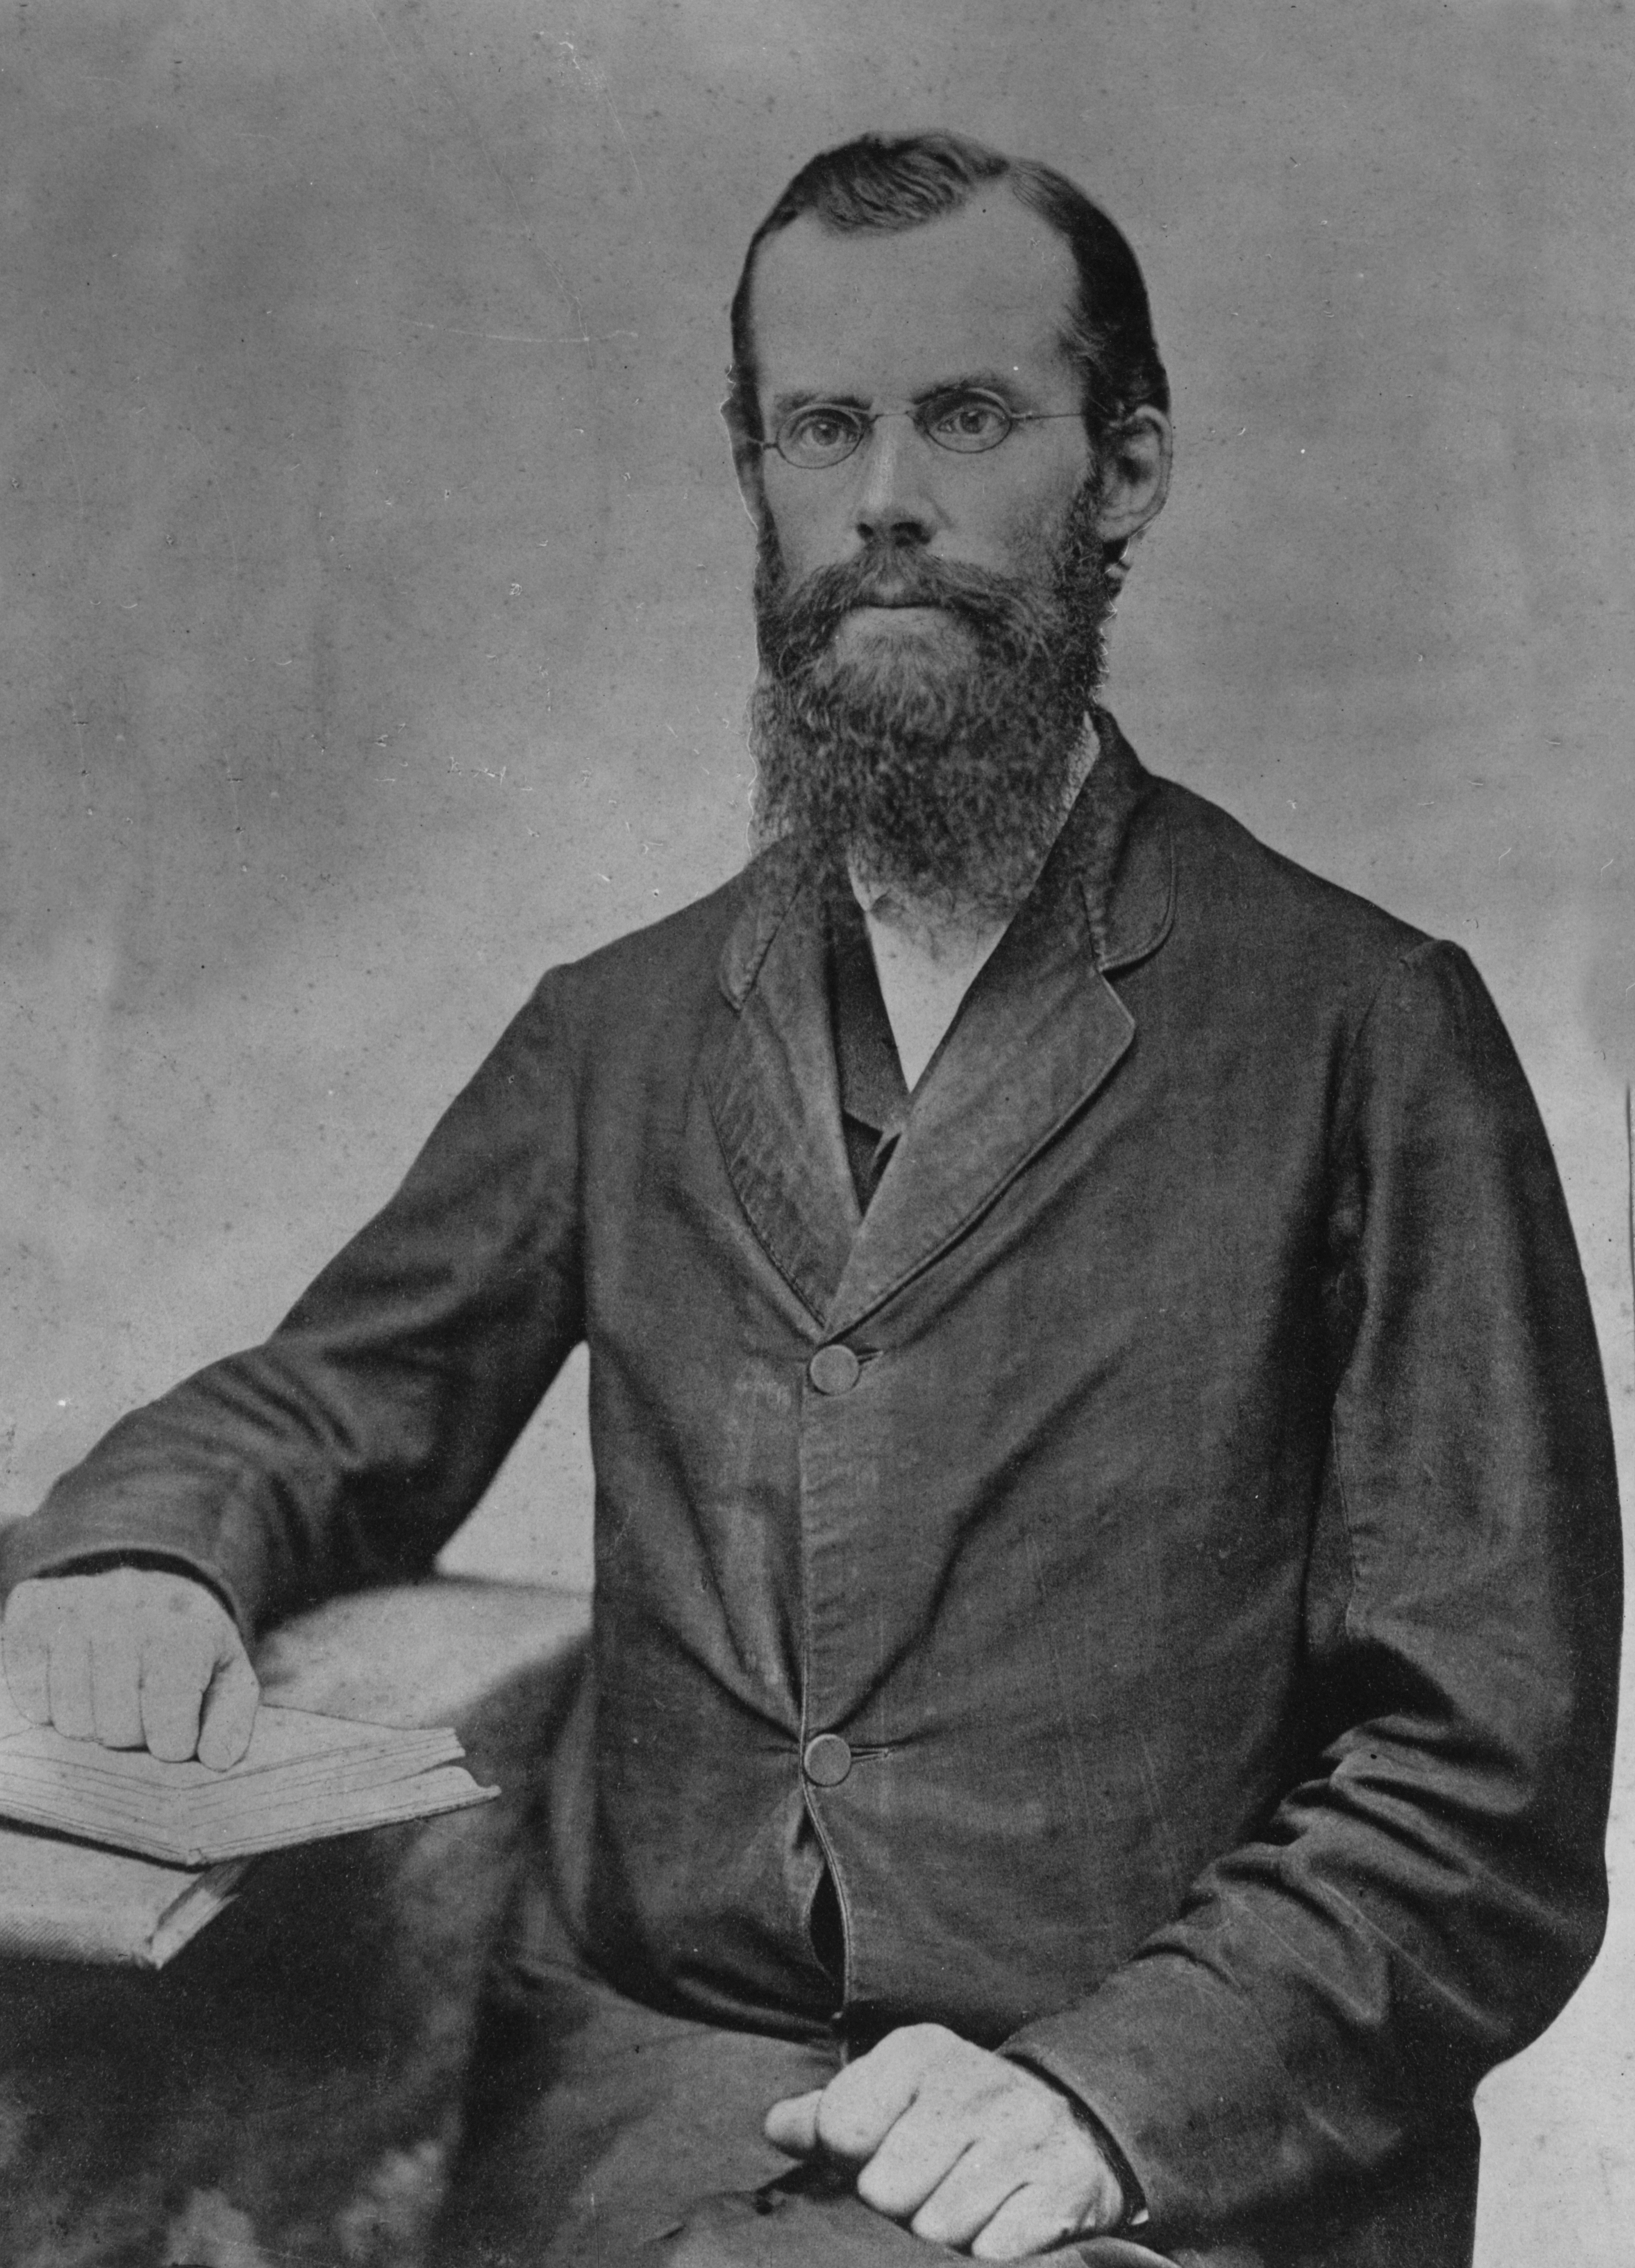
\includegraphics[width=1\linewidth]{images/john-nevins-andrews.jpg}
    \caption*{John Nevins Andrews (1829-1883)}
    \label{fig:j-n-andrews}
\end{figure}


\begin{figure}[hp]
    \centering
    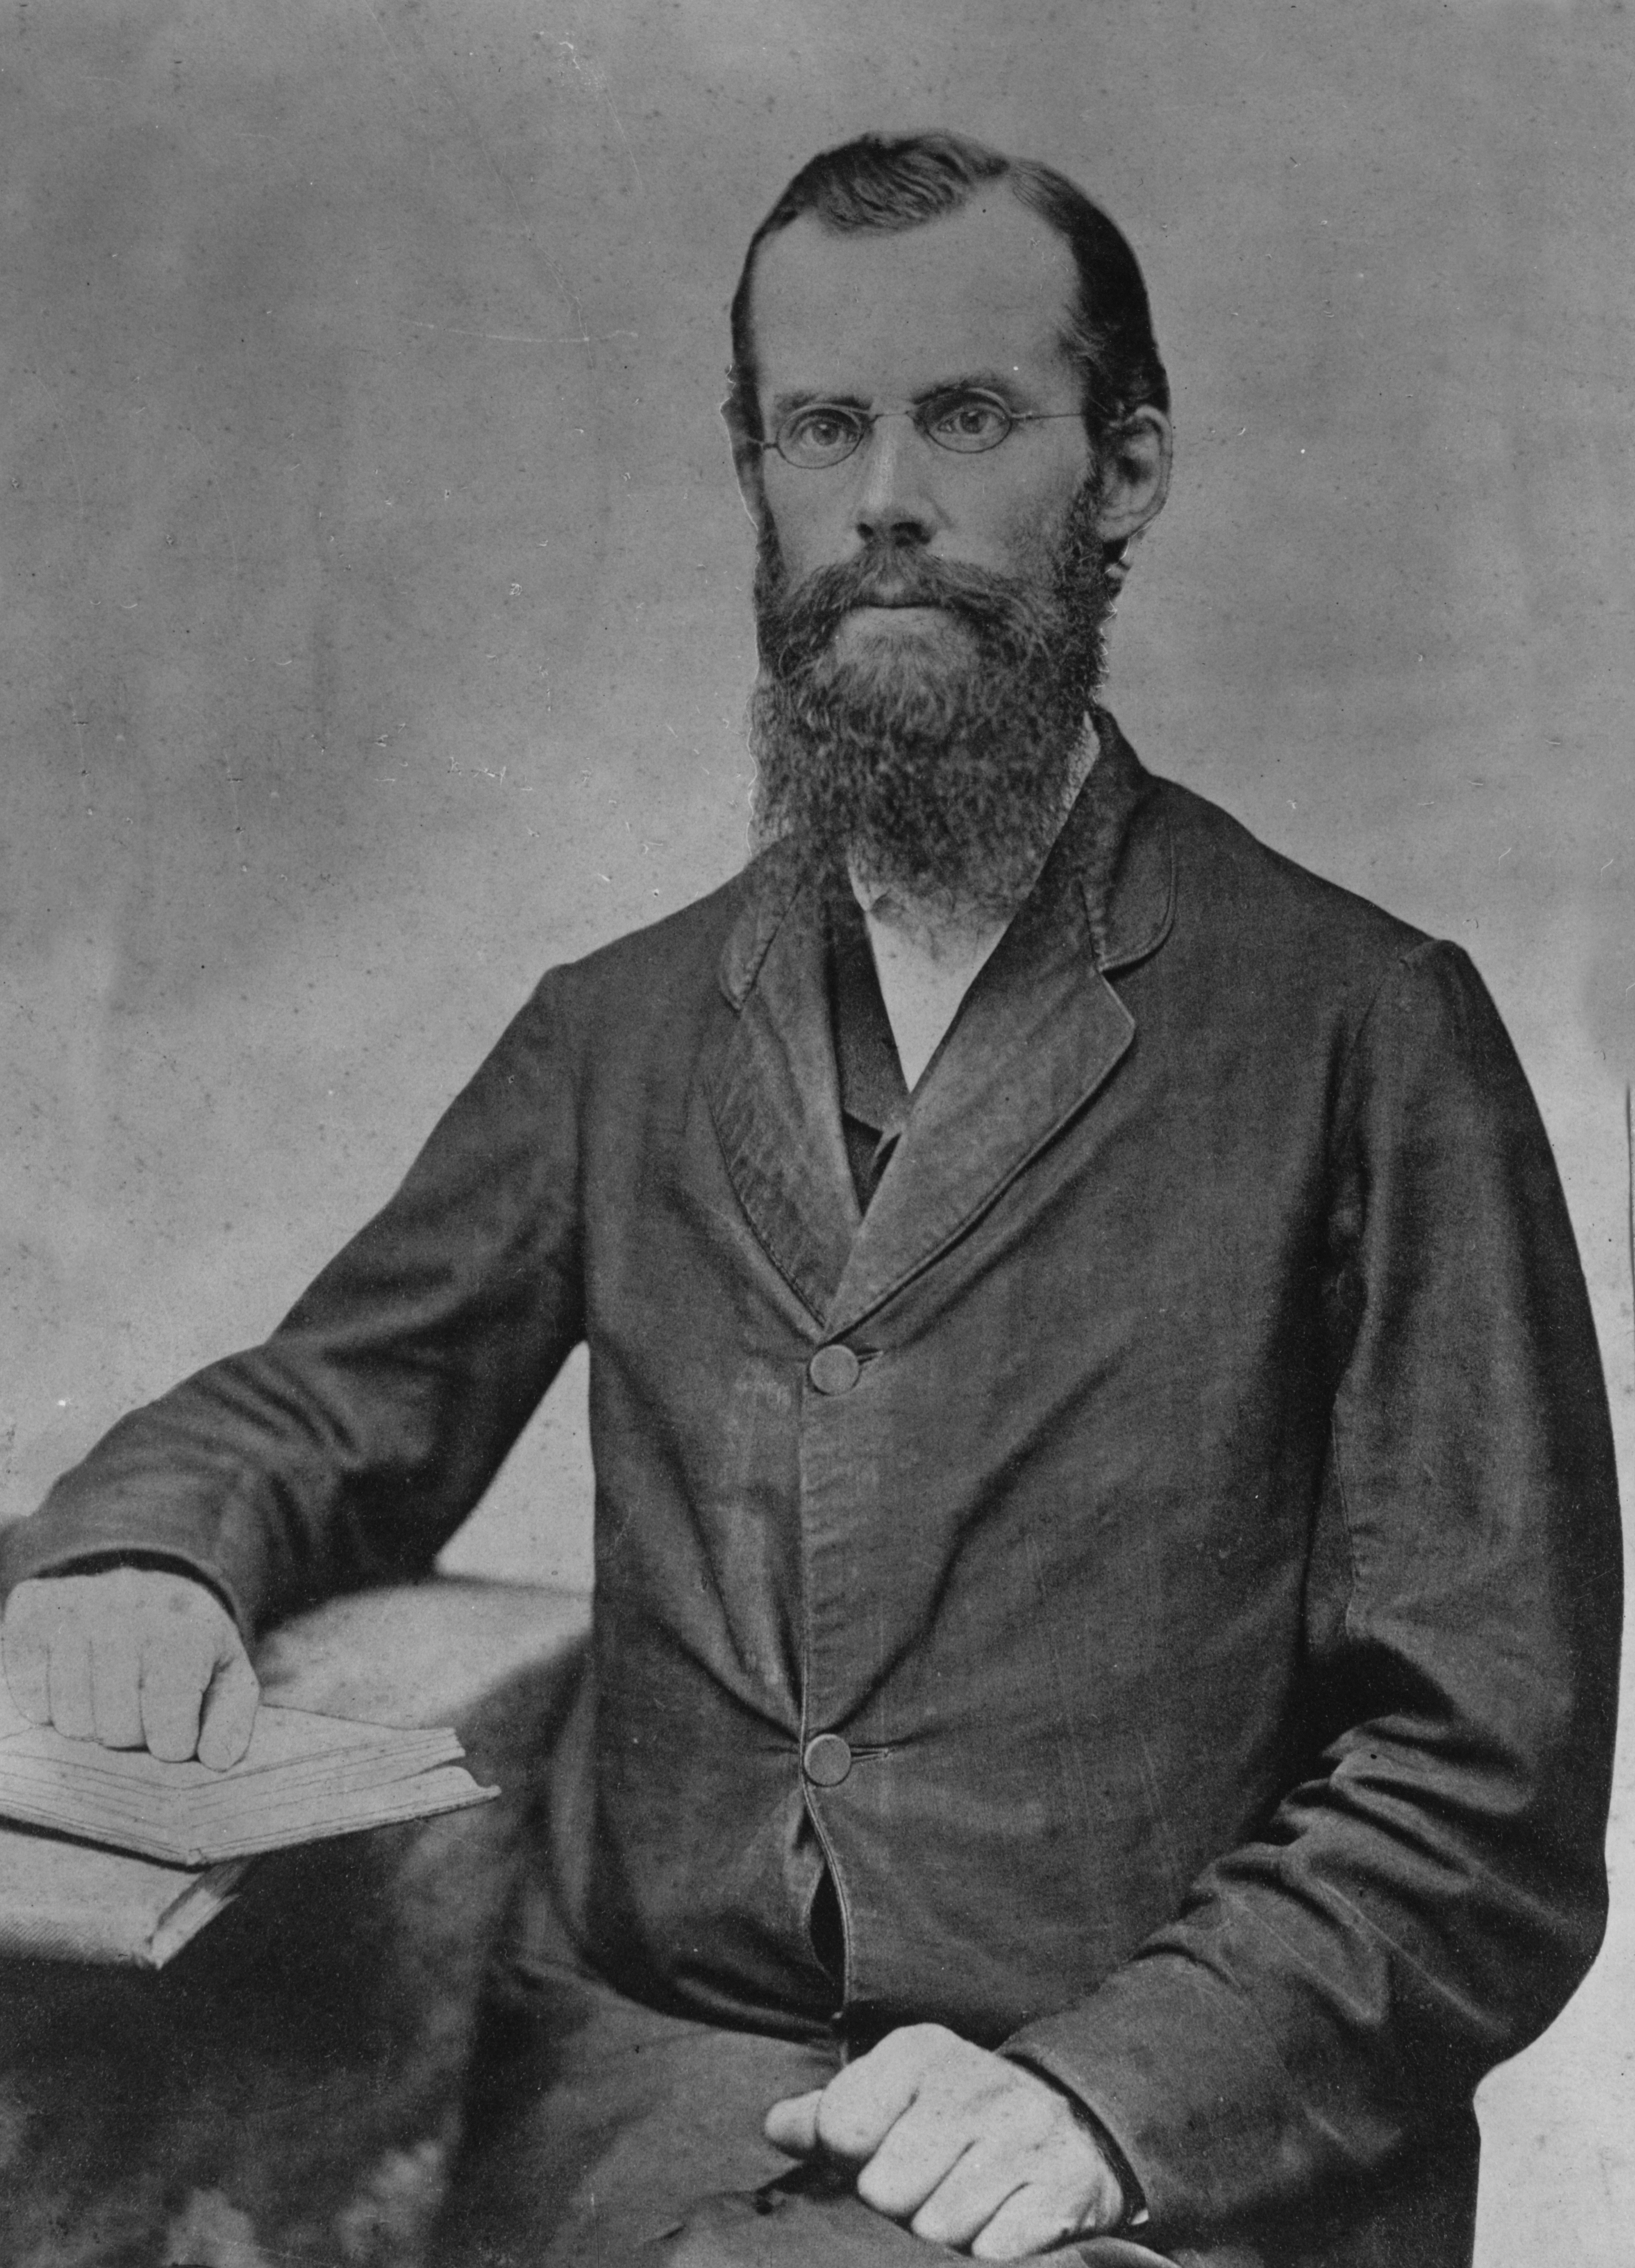
\includegraphics[width=1\linewidth]{images/john-nevins-andrews.jpg}
    \caption*{John Nevins Andrews (1829-1883)}
    \label{fig:j-n-andrews}
\end{figure}


J. N. Andrews said, \others{\textbf{The doctrine of the Trinity which was established in the church by the council of Nicea, A. D. 325}. \textbf{This doctrine \underline{destroys the personality of God, and his Son Jesus Christ our Lord}}...}[John. N. Andrews, The Advent Review and Sabbath Herald, March 6, 1855, p. 185][http://documents.adventistarchives.org/Periodicals/RH/RH18550306-V06-24.pdf]


J. N. Andrews alisema, \others{\textbf{Fundisho la Utatu ambalo lilianzishwa katika kanisa na Baraza la Nicea, A. D. 325}. \textbf{Fundisho hili \underline{linaharibu Umbile la Mungu, na Mwana Yesu Kristo Bwana wetu}}...}[John. N. Andrews, The Advent Review and Sabbath Herald, March 6, 1855, p. 185][http://documents.adventistarchives.org/Periodicals/RH/RH18550306-V06-24.pdf]


In the context of the trinitarian understanding of the \emcap{personality of God}, it is safe to say that the \emcap{personality of God}, or the quality or state of God being a person, in any understanding of Trinity doctrine is a mystery. The problem is that there is no clear view of who is that \textit{one God} who is a person? The underlying claim is made that God is One yet Three, or One in Three; yes, God is a person, and He is one, yet simultaneously He is three persons. This view can never hold any clear perception of the \emcap{personality of God}. Also, it will deny the clearest testimony of the Scriptures that the one God is the Father, and that Christ is truly His only begotten Son. Most trinitarian brothers would agree that Christ is a real and definite being but if a trinitarian were to accept the Father as a real and definite Being, he would also need to accept the Holy Spirit as a real and definite being, thus denying the Holy Spirit as being a \textit{spirit}, the means by which the Father and Son are omnipresent. Conversely, if a trinitarian accepted the Holy Spirit to be a literal spirit, having no body nor form, then he would deny the Father to be a real, definite being. In conversation over the quality or state of God being a person, there is never a clear view of the matter with promoters of the Trinity doctrine; it is subterfuge. \textit{‘Subterfuges’} is a word Sister White used to describe the deception by artifice or stratagem in order to conceal, escape, or evade\footnote{\href{https://www.merriam-webster.com/dictionary/subterfuges}{The Merriam-Webster, ‘subterfuges’} - “\textit{deception by artifice or stratagem in order to conceal, escape, or evade}”} the truth; in other words, something that you cannot grab by head or tail. This is the primary reason Sister White did not engage in the Trinity discussion that would come up in the Seventh-day Adventist Church.


Katika muktadha wa ufahamu wa utatu kuhusu Umbile la Mungu, ni salama kusema kwamba Umbile la Mungu, au Ubora au hali ya Mungu kuwa Nafsi, katika ufahamu wowote ule wa Fundisho la Utatu ni swala lililo fumbo. Shida ni kwamba hakuna maoni wazi ya nani huyo \textit{Mungu mmoja} ambaye ni nafsi? Dai la msingi linafanywa kwamba Mungu ni Mmoja bado ni Watatu, au Mmoja ndani Tatu; ndio, Mungu ni Nafsi, na Yeye ni mmoja, lakini wakati huo huo Yeye ni nafsi tatu. Hii mtazamo hauwezi kamwe kushikilia mtazamo wowote wazi wa Umbile la Mungu. Pia, itakataa ushuhuda wa wazi kabisa wa Maandiko kwamba Mungu mmoja ndiye Baba, na kwamba Kristo ndiye kweli Mwana wake wa pekee. Ndugu wengi wa utatu wangekubali kwamba Kristo ni halisi na wa uhakika lakini ikiwa mwamini-utatu angemkubali Baba kama Halisi halisi na dhahiri, angemkubali pia Roho Mtakatifu kama Huluki halisi na dhahiri, hivyo kumkana Roho Mtakatifu kama kuwa \textit{roho}, njia ambayo kwayo Baba na Mwana wako kila mahali. Kinyume chake, ikiwa wa utatu wangemkubali Roho Mtakatifu kuwa Roho halisi, asiye na mwili wala umbo, basi yeye angemkana Baba kuwa Huluki halisi na dhahiri. Katika mazungumzo juu ya Ubora au hali ya Mungu kuwa Nafsi, hakuna kamwe maoni wazi ya jambo hilo kutoka kwa waendelezaji wa mafundisho ya Utatu; ni hila. \textit{‘Hila’} ni neno ambalo Dada White alitumia kuelezea udanganyifu huo wa usanii au ili kuficha, kuepuka, au kukwepa\footnote{\href{https://www.merriam-webster.com/dictionary/subterfuges}{The Merriam-Webster, ‘subterfuges’} - “\textit{deception by artifice or stratagem in order to conceal, escape, or evade}”} ukweli; kwa maneno mengine, kitu ambacho huwezi kunyakua kwa kichwa au mkia. Hii ndiyo sababu kuu ya Dada White kufanya kutojihusisha na majadiliano ya Utatu ambayo yangetokea katika kanisa la Waadventista Wasabato.


\egw{I was cautioned not to enter into controversy \textbf{regarding the question} that \textbf{\underline{will come up}} over \textbf{these things, because controversy \underline{might lead men to resort to subterfuges, and their minds would be led away from the truth of the Word of God to assumption and guesswork}}. \textbf{The more that fanciful theories are discussed, the \underline{less men will know of God and of the truth that sanctifies the soul}}.}[Lt232-1903.41; 1903][https://egwwritings.org/read?panels=p10197.50]


\egw{Nilitahadharishwa nisiingie kwenye mabishano \textbf{kuhusiana na swali} litakalo\textbf{\underline{jitokeza}} juu ya \textbf{mambo haya, kwa sababu mabishano yanaweza \underline{kusababisha watu kutumia hila, na akili zao zingeongozwa mbali na kweli wa Neno la Mungu hadi kwenye dhana na kazi ya kubahatisha}}. \textbf{Kadiri nadharia potofu zinavyojadiliwa, \underline{ndivyo wanadamu watakavyojua kidogo kuhusu Mungu na wa ile kweli inayotakasa nafsi}}.}[Lt232-1903.41; 1903][https://egwwritings.org/read?panels=p10197.50]


When we read the works of Seventh-day Adventist pioneers on the \emcap{personality of God}, we see that they did not fall into the Trinity trap. Their non-trinitarian views of God were not due to ignorance, but a knowledge of the truth on the \emcap{personality of God}. They were of keen and noble intellect, understanding the thin line between the truth and error. Their understanding of the \emcap{personality of God} is balanced and solid, strongly supported by the plain and simple “\textit{thus says the Lord}”.


Tunaposoma kazi za waanzilishi wa Waadventista Wasabato juu ya Umbile la Mungu, tunaona kwamba hawakuanguka katika mtego wa Utatu. Maoni yao yasiyo ya utatu juu ya Mungu hayakukwa juu ya kutokwa na hekima, bali ujuzi wa ukweli juu ya Umbile la Mungu. Walikuwa na nia na akili nzuri, kuelewa mstari mwembamba kati ya ukweli na makosa. Uelewa wao wa Umbile la Mungu umelingana na kutoshana na kipimio, inaungwa mkono kwa nguvu kwa tamko lililo rahisi na wazi “\textit{Bwana asema hivi}”.


Many Adventists today accept the Trinity doctrine because Ellen White supposedly accepted it and promoted it. This is far from the truth and such a conclusion is predicated on lacking knowledge of the Spirit of Prophecy. If anyone was acquainted with the beliefs of Sister White, it was her husband James White. Here is what he has to say about the writings of his wife:


Waadventista wengi leo wanakubali fundisho la Utatu kwa sababu Ellen White kwa madhanio ya watu, alikuja kuikubali na kuikuza. Hii ni mbali na ukweli na hitimisho kama hilo linatabiriwa kukosa ujuzi wa Roho ya Unabii. Ikiwa mtu yeyote alikuwa anafahamu imani za Dada White, alikuwa mume wake James White. Hapa kuna anachosema juu ya maandishi ya mke:


\others{\textbf{We invite all to compare the testimonies of the Holy Spirit through Mrs. W., with the word of God}. \textbf{And in this we do not invite you to compare them \underline{with your creed}}. That is quite another thing. \textbf{\underline{The trinitarian may compare them with his creed, and because they do not agree with it, condemn them}}. The observer of Sunday, or the man who holds eternal torment an important truth, and the minister that sprinkles infants, may each condemn the testimonies’ of Mrs. W. because they do not agree with their peculiar views. And a hundred more, each holding different views, may come to the same conclusion. \textbf{But their genuineness can never be tested in this way}.}[James S. White, The Advent Review, and Herald of the Sabbath, June 13, 1871][https://documents.adventistarchives.org/Periodicals/RH/RH18710613-V37-26.pdf]


\others{\textbf{Tunawaalika wote kulinganisha shuhuda za Roho Mtakatifu kupitia Bi. W., na neno la Mungu}. \textbf{Na katika hili hatukualiki kulinganisha \underline{na itikadi yako}}. Hiyo ni jambo jingine kabisa. \textbf{\underline{Mwenye kuamini utatu anaweza kuzilinganisha na imani yake, na kwa sababu hazikubaliani nayo, wanatoa hukumu}}. Anayeomba Jumapili, au mtu anayeshikilia mateso ya milele kama ukweli muhimu, na mtumishi anayenyunyizia watoto wachanga kwa ubatizo, wanaweza kila mmoja wao kulaani shuhuda’ za Bi. W. kwa sababu hazikubaliani na maoni yao ya kipekee. Na mia zaidi, kila mmoja akiwa na maoni tofauti, anaweza kufikia mkataa uleule. \textbf{Lakini uhalisi wao kamwe hauwezi kujaribiwa kwa namna hii}.}[James S. White, The Advent Review, and Herald of the Sabbath, June 13, 1871][https://documents.adventistarchives.org/Periodicals/RH/RH18710613-V37-26.pdf]


James White was the closest associate of Ellen White, the person who was one with her in God’s uplifting of the Seventh-day Adventist Church. We have a clear and direct testimony from him that Ellen White’s writings are not trinitarian. Today, scholars put a false narrative that Ellen White grew in her understanding of the Trinity doctrine, and eventually accepted and preached it. But we see that Ellen White did not change her standpoint on the \emcap{personality of God} nor did she adhere to the Trinity doctrine. She was unambiguous in her claim that she never did. When the Kellogg crisis came over the \emcap{personality of God}, she remained firm in her view, just as all early Seventh-day Adventist pioneers did—and her dealings with Dr. Kellogg prove that. It is true, the Trinity doctrine \textit{cannot be accepted by those who are loyal to the faith and to the principles that have withstood all the opposition of satanic influences}.\footnote{\egw{Patchwork theories cannot be accepted by those who are loyal to the faith and to the principles that have withstood all the opposition of satanic influences}[Lt253-1903.28; 1903][https://egwwritings.org/read?panels=p14068.9980036]} Today’s official narrative that Ellen White was teaching the Trinity echoes Dr. Kellogg’s claim that the Living Temple taught the same thing as Ellen White. \egwinline{\textbf{But God forbid that this sentiment should prevail}.}[SpTB02 53.3; 1904][https://egwwritings.org/read?panels=p417.272]


James White alikuwa mshirika wa karibu zaidi wa Ellen White, mtu ambaye alikuwa mmoja naye katika kuliinua Kanisa la Waadventista Wasabato. Tuna ushuhuda wa wazi na wa moja kwa moja kutoka kwake kwamba maandishi ya Ellen White si ya utatu. Leo, wasomi huweka hadithi za uwongo kwamba Ellen White alikua katika ufahamu wake wa fundisho la Utatu, na hatimaye akakubali na kuihubiri. Lakini tunaona kwamba Ellen White hakubadilisha maoni yake juu ya Umbile la Mungu wala hakushikamana na fundisho la Utatu. Alikuwa wazi ndani yake kudai kwamba hakuwahi kufanya hivyo. Wakati mzozo wa Kellogg ulipokuja juu ya Umbile la Mungu, yeye alibaki imara katika maoni yake, kama vile mapainia wote wa mapema wa Waadventista Wasabato walivyofanya—na mahusiano yake na Dk. Kellogg yanathibitisha hilo. Ni kweli, fundisho la Utatu \textit{haliwezi kukubaliwa na wale ambao ni waaminifu kwa imani na kwa kanuni ambazo zimestahimili upinzani wote wa ushawishi wa kishetani}.\footnote{\egw{Nadharia za Kiraka haziwezi kukubaliwa na wale ambao ni waaminifu kwa imani na kwa kanuni ambazo zimestahimili upinzani wote wa ushawishi wa kishetani}[Lt253-1903.28; 1903][https://egwwritings.org/read?panels=p14068.9980036]} Simulizi rasmi ya leo kwamba Ellen White alikuwa akifundisha Utatu inaangazia madai ya Dk. Kellogg kwamba The Living Temple ilifundisha kitu sawa na Ellen White. \egwinline{\textbf{Lakini Mwenyezi Mungu apishe mbali hisia hii kuwa na nguvu}.}[SpTB02 53.3; 1904][https://egwwritings.org/read?panels=p417.272]


% Adventist pioneers and the Trinity doctrine

\begin{titledpoem}
    \stanza{
        The pioneers stood firm against the Trinity's sway, \\
        Their testimony clear as the light of day. \\
        They saw how this doctrine did subtly disguise, \\
        What Scripture reveals to discerning eyes.
    }

    \stanza{
        James White declared it among "popular fables" found, \\
        A teaching that makes God's personality unsound. \\
        For Father and Son as distinct beings stand, \\
        Not merged into one as the Trinity planned.
    }

    \stanza{
        Two separate persons with purpose aligned, \\
        In spirit and action, united in mind. \\
        Just as disciples in Christ become one, \\
        Yet remain individual under God's Son.
    }

    \stanza{
        The Holy Spirit, God's presence divine, \\
        Not a separate being of the Godhead's design. \\
        But truly God's Spirit sent forth from above, \\
        The Father's representative, agent of love.
    }

    \stanza{
        No Scripture supports what tradition declared, \\
        When at Nicea this doctrine was shared. \\
        John seventeen shatters the trinitarian view, \\
        Revealing the Father and Son as beings true.
    }

    \stanza{
        Christ's divinity rests not in mysterious three, \\
        But in His begotten Sonship we see. \\
        The express image of His Father's face, \\
        Inheriting fullness of divine grace.
    }

    \stanza{
        The pioneers knew what the Bible made clear, \\
        That God is the Father, a Being most dear. \\
        A personal, spiritual presence on high, \\
        Omnipresent through Spirit, yet dwelling on high.
    }

    \stanza{
        So stands the truth against error's long night, \\
        Preserved by the pioneers and Sister White. \\
        Not through confusion or mystical thought, \\
        But through plain Scripture the truth has been taught.
    }
\end{titledpoem}


% Adventist pioneers and the Trinity doctrine

\begin{titledpoem}
    \stanza{
        The pioneers stood firm against the Trinity's sway, \\
        Their testimony clear as the light of day. \\
        They saw how this doctrine did subtly disguise, \\
        What Scripture reveals to discerning eyes.
    }

    \stanza{
        James White declared it among "popular fables" found, \\
        A teaching that makes God's personality unsound. \\
        For Father and Son as distinct beings stand, \\
        Not merged into one as the Trinity planned.
    }

    \stanza{
        Two separate persons with purpose aligned, \\
        In spirit and action, united in mind. \\
        Just as disciples in Christ become one, \\
        Yet remain individual under God's Son.
    }

    \stanza{
        The Holy Spirit, God's presence divine, \\
        Not a separate being of the Godhead's design. \\
        But truly God's Spirit sent forth from above, \\
        The Father's representative, agent of love.
    }

    \stanza{
        No Scripture supports what tradition declared, \\
        When at Nicea this doctrine was shared. \\
        John seventeen shatters the trinitarian view, \\
        Revealing the Father and Son as beings true.
    }

    \stanza{
        Christ's divinity rests not in mysterious three, \\
        But in His begotten Sonship we see. \\
        The express image of His Father's face, \\
        Inheriting fullness of divine grace.
    }

    \stanza{
        The pioneers knew what the Bible made clear, \\
        That God is the Father, a Being most dear. \\
        A personal, spiritual presence on high, \\
        Omnipresent through Spirit, yet dwelling on high.
    }

    \stanza{
        So stands the truth against error's long night, \\
        Preserved by the pioneers and Sister White. \\
        Not through confusion or mystical thought, \\
        But through plain Scripture the truth has been taught.
    }
\end{titledpoem}
